\documentclass[a4paper,11pt]{article}

% -------------------------------------------------------
% Packages
% -------------------------------------------------------
\usepackage{amsmath,amssymb}
\usepackage{graphicx}
\usepackage{geometry}
\usepackage{hyperref}
\usepackage{bm}
\usepackage{physics}
\usepackage{tikz}
\geometry{margin=2.5cm}

% Hyperlink settings
\hypersetup{
    colorlinks = true,
    linkcolor = blue,
    citecolor = blue,
    urlcolor  = blue
}

% -------------------------------------------------------
\begin{document}

\title{\textbf{Energy-Flow Cosmology}\\[4pt]
Unified Model Specification (Master Document)}
\author{Morten Magnusson}
\date{\today}
\maketitle

\tableofcontents
\newpage

% -------------------------------------------------------
\section{Introduction}

This master document compiles the full formal structure of Energy-Flow
Cosmology (EFC). It unifies the dynamical sector (EFC-D), the structural
sector (EFC-S), observable predictions, and optional diagrams into a
single cohesive specification.

The master file acts as the top-level entry point for the full theory
and can be compiled directly using the GitHub PDF pipeline.

% -------------------------------------------------------
\newpage
\section{EFC-D: Dynamical Sector}
% ===========================================================
% EFC-D: Energy-Flow Dynamics
% ===========================================================

\section*{EFC-D: Energy-Flow Potential}

The local energy-flow potential $E_f$ is defined as a function of
mass density $\rho$ and entropy $S$:

\[
E_f = \rho \,(1 - S)
\]

This expresses:

\begin{itemize}
    \item High density and low entropy $\rightarrow$ large $E_f$
    \item High entropy $\rightarrow$ suppresses $E_f$
\end{itemize}

% -----------------------------------------------------------
% 1. Density
% -----------------------------------------------------------
\subsection*{1. Density}

The mass density is defined as:

\[
\rho = \frac{m}{V}
\]

where $m$ is the mass contained in the local region and $V$ is the
corresponding volume.

% -----------------------------------------------------------
% 2. Energy-Flow Rate
% -----------------------------------------------------------
\subsection*{2. Energy-Flow Rate}

The temporal change in the energy-flow potential is:

\[
\frac{dE_f}{dt} = \nabla_t E_f
\]

This represents the local rate of change in the potential along the
temporal direction.

% -----------------------------------------------------------
% Reference to source code
% -----------------------------------------------------------
\subsection*{Code Reference}

The computational implementation is available in:

\begin{verbatim}
src/efc_potential.py
\end{verbatim}


% -------------------------------------------------------
\newpage
\section{EFC-S: Structural Sector}
\section{EFC-S: Entropy Field and Gradient}

The EFC-S sector defines the entropy field $S(\mathbf{x})$.
This field encodes local structural organization and acts as a
non-mass-based driver of curvature-like behavior.

\subsection{Entropy Field}

The entropy field is treated as a scalar function:
\begin{equation}
    S : \mathbb{R}^3 \rightarrow [S_{\min}, S_{\max}].
\end{equation}

The field can be interpreted as a measure of information or
organizational density in configuration space.

\subsection{Entropy Gradient}

The entropy gradient is:
\begin{equation}
    \nabla S(\mathbf{x}) = 
    \left(
      \frac{\partial S}{\partial x},
      \frac{\partial S}{\partial y},
      \frac{\partial S}{\partial z}
    \right).
\end{equation}

The scaled physical gradient used in the model is:
\begin{equation}
    \mathbf{g}_S = k_S \nabla S.
\end{equation}

This gradient introduces directional asymmetry which couples
to the energy-flow field and affects structure formation.


% -------------------------------------------------------
\newpage
\section{Observables and Light Propagation}
\section{Observables and Validation Mapping}

\subsection{JWST}

EFC predicts early galaxy presence via the 
$(E_f, S)$-dependent structural growth rate.

\subsection{DESI / BAO}

The expansion curve derived from $H(E_f,S)$ maps to 
$H(z)$ and BAO observables.

\subsection{SPARC}

The circular velocity is given by:
\begin{equation}
    v(r) = \sqrt{r \frac{\partial \Phi}{\partial r}}.
\end{equation}

This provides direct comparison with rotation curve datasets.


% -------------------------------------------------------
\newpage
\section{Light-Dynamics and Endpoint Behaviour (s$_0$–s$_1$)}
% ============================================================
% EFC-C₀: Entropy-Dependent Light Propagation
% ============================================================

\section{EFC-C\textsubscript{0}: Entropy-Dependent Light Propagation}
\label{sec:efc_c0}

Energy-Flow Cosmology treats the effective speed of light as an
emergent property of the thermodynamic state of the grid. The
field $S(\mathbf{x})$ does not only modulate structure and
energy-flow, but also the propagation of information.

EFC-C\textsubscript{0} closes the chain
\[
  S(\mathbf{x})
  \;\Rightarrow\;
  E_f(\mathbf{x})
  \;\Rightarrow\;
  \Phi(E_f,S)
  \;\Rightarrow\;
  c(S)
  \;\Rightarrow\;
  H(E_f,S)
  \;\Rightarrow\;
  \text{Observables}.
\]

% ------------------------------------------------------------
\subsection{Entropy Endpoints and Normalised Coordinate}

We define two entropy endpoints
\begin{itemize}
  \item $s_0$: low-entropy, high-structure endpoint,
  \item $s_1$: high-entropy, high-diffusion endpoint,
\end{itemize}
with midpoint and span
\[
  S_{\text{mid}} = \frac{1}{2}(s_0 + s_1),
  \qquad
  \Delta S = s_1 - s_0.
\]

A normalised entropy coordinate is
\[
  x(S) = \frac{S - S_{\text{mid}}}{\Delta S/2},
\]
so that $x = -1$ corresponds to $S = s_0$ and $x = +1$ to $S = s_1$.

% ------------------------------------------------------------
\subsection{Effective Speed of Light and Refractive Index}

The effective speed of light is modeled as an even function around
$S_{\text{mid}}$:
\[
  c(S) = c_0 \left( 1 + a_{\text{edge}}\, x(S)^2 \right),
\]
where $a_{\text{edge}}$ controls the strength of edge-driven
modulation. The corresponding refractive index is
\[
  n(S) = \frac{c_0}{c(S)}
       = \frac{1}{1 + a_{\text{edge}}\, x(S)^2}.
\]

In the EFC grid frame, $c_0$ is the reference value in a
weakly-structured, mid-entropy background. Deviations are entirely
encoded in $S$.

% ------------------------------------------------------------
\subsection{Light Travel Time and Fermat Principle}

For a photon trajectory $\gamma$ the observed travel time is
\[
  t_{\text{obs}}
  = \int_{\gamma} \frac{dl}{c(S(l))}
  = \frac{1}{c_0} \int_{\gamma} n\bigl(S(l)\bigr)\, dl.
\]

The path is determined by a thermodynamic Fermat principle:
\[
  \delta \int_{\gamma} n\bigl(S(\mathbf{x})\bigr)\, dl = 0.
\]

Gradients in $S$ therefore act as an effective refractive medium,
even at fixed mass distribution.

% ------------------------------------------------------------
\subsection{Dual Focusing–Defocusing Behaviour}

The entropy endpoints have distinct optical roles:
\begin{itemize}
  \item Near $s_0$ (low entropy, strong structure) the local
    modulation of $c(S)$ and $n(S)$ produces focusing similar to
    mass overdensities.
  \item Near $s_1$ (high entropy, loosened structure) the same
    mechanism generates large-scale defocusing.
  \item Around $S_{\text{mid}}$ the propagation is slowest, giving
    maximal time delays.
\end{itemize}

This yields a dual-lens profile:
\begin{align*}
  s_0 &\;\Rightarrow\; \text{sharp, local focusing}, \\
  s_1 &\;\Rightarrow\; \text{broad, diffuse defocusing}.
\end{align*}

% ------------------------------------------------------------
\subsection{Coupling to the EFC Potential and Expansion}

Because $S(\mathbf{x})$ also controls the energy-flow potential
\(
  E_f = \rho(1-S)
\),
the same field that modulates $c(S)$ drives the potential
$\Phi(E_f,S)$ and the expansion rate
\[
  H(E_f,S) = \sqrt{|E_f|}\,(1+S).
\]

In EFC-C\textsubscript{0}, apparent anomalies in
\begin{itemize}
  \item lensing strength,
  \item time-delay ratios,
  \item inferred distances and expansion rates,
\end{itemize}
are interpreted as consequences of entropy-structured
light propagation rather than missing mass or a separate dark energy
component.


% -------------------------------------------------------
\newpage
\section{Flow Diagrams (Optional)}
\begin{center}
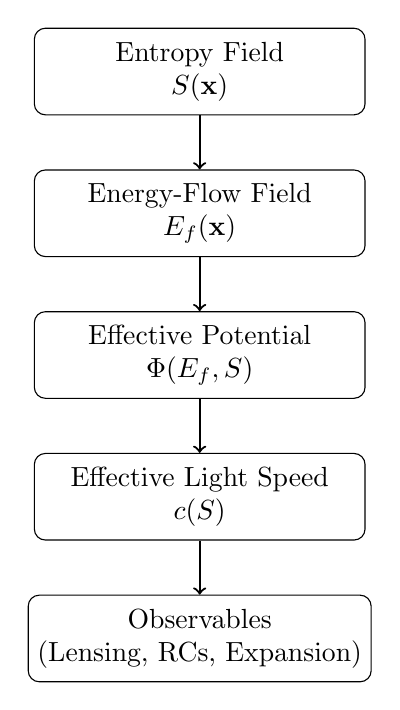
\begin{tikzpicture}[
    node distance=1.8cm,
    box/.style={
        rectangle,
        draw=black,
        rounded corners,
        minimum width=4.2cm,
        minimum height=1.1cm,
        align=center
    },
    arrow/.style={->, thick}
]

% Nodes
\node[box] (S)         {Entropy Field \\ $S(\mathbf{x})$};
\node[box, below of=S] (Ef)        {Energy-Flow Field \\ $E_f(\mathbf{x})$};
\node[box, below of=Ef] (Phi)     {Effective Potential \\ $\Phi(E_f,S)$};
\node[box, below of=Phi] (cS)     {Effective Light Speed \\ $c(S)$};
\node[box, below of=cS] (Obs)     {Observables \\ (Lensing, RCs, Expansion)};

% Arrows
\draw[arrow] (S)   -- (Ef);
\draw[arrow] (Ef)  -- (Phi);
\draw[arrow] (Phi) -- (cS);
\draw[arrow] (cS)  -- (Obs);

\end{tikzpicture}
\end{center}


% -------------------------------------------------------
\newpage
\section{Appendix: Equations Summary}
\section{Core Equations of EFC}

\subsection{Entropy Structure}
\[
S_{\text{mid}} = \frac{1}{2}(S_0+S_1), \qquad
\Delta S = S_1-S_0,
\qquad
x(S)=\frac{S-S_{\text{mid}}}{\Delta S/2}.
\]

\subsection{Effective Light Speed}
\[
c(S) = c_0 \left(1 + a_{\text{edge}} x(S)^2\right).
\]

\subsection{Energy Flow and Potential}
\[
E_f \propto -\nabla S,
\qquad
\Phi(E_f,S)=A_\Phi E_f(1+S).
\]

\subsection{Expansion Rate}
\[
H(E_f,S)=\sqrt{|E_f|}(1+S).
\]

\subsection{Rotation Curves}
\[
v(r)=\sqrt{r\frac{\partial \Phi}{\partial r}}.
\]

\subsection{Light-Travel Time}
\[
t_{\text{obs}}=\int_\gamma \frac{dl}{c(S(l))}.
\]


% -------------------------------------------------------
\end{document}
